\section{Introduction}
\label{sec:introduction}

% state the learning objective 
The objective of this laboratory assignment is to study a circuit containing a
sinusoidal voltage source $V_I$ connected to a resistor $R$ and a capacitor $C$
in series. The circuit can be seen if Figure~\ref{fig:rc}.

In Section~\ref{sec:analysis}, a theoretical analysis of the circuit is
presented. In Section~\ref{sec:simulation}, the circuit is analysed by
simulation, and the results are compared to the theoretical results obtained in
Section~\ref{sec:analysis}. The conclusions of this study are outlined in
Section~\ref{sec:conclusion}.

\begin{figure}[h] \centering
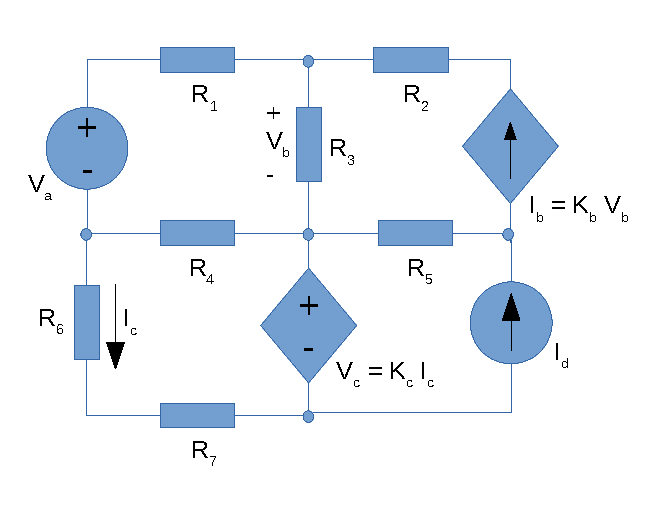
\includegraphics[width=0.4\linewidth]{rc.pdf}
\caption{Voltage driven serial RC circuit.} %mudar legendaaaaaaaaaaa!!!!!!
\label{fig:rc}
\end{figure}


\begin{center}


Where:

$R_1 = 1.03431507833 $

$R_2 = 2.02853090731$
 
$R3 = 3.1462050633 $

$R_4 = 4.03438547455$ 

$R_5 = 3.12170042214 $

$R_6 = 2.07116379646 $

$R_7 = 1.01597753093 $

$V_a = 5.156959346 $

$I_d = 1.01455683569 $

$K_b = 7.1497941196 $

$K_c = 8.12593642585 $
\end{center}

Units for the values: $V, mA, k\Omega$ and $mS$



